\chapter{タスク3：切断時の安定把持}
% ============================================================
\label{ch:holding}
% ============================================================

% ------------------------------------------------------------
\section{問題設定と本章の位置づけ}
\label{sec:holding_problem_and_role}
% ------------------------------------------------------------

\subsection{本章の位置づけ}
\label{subsec:holding_position}

\revise{本章は，第1章で整理した形状，力学，環境・道具という分析観点を，包丁による食材切断中の把持点選択へ適用した事例である．}

第3章で述べた3Dモデル取得基盤の上に，本章では食材表面上での把持点探索と包丁外力下での力学解析を積み上げ，双腕ロボットによる把持・切断動作の実行へと接続する．

本タスクは，包丁から食材に加わる力とトルクに抗して食材の意図しない移動を防ぐ{\nameholdingpointset}を，食材の三次元形状と包丁軌道を入力として解析的に算出する問題として定式化される．

\begin{revisionblock}
\subsection{想定する状況，目的および達成範囲}
本章は，家庭で食材を包丁により所定の位置で切断する際に，他方の手で食材を押さえて横滑りや回転を防ぐ操作を想定する．
ロボットには切断位置と包丁の往復軌道，指本数，食材種別に対応する破壊靭性・圧力分布・摩擦係数が既知または事前計測値として与えられ，食材表面の3D点群から安全かつ力学的に成立する接触位置を決定する．
実験では，まな板と安定な平面接触を持つ半切りのジャガイモおよび玉ねぎを対象とし，把持位置は切断前にオフラインで計算する．
食材・包丁の選択，切断軌道自体の自動生成，食材物性のオンライン推定，刃先周辺の人に対する安全監視，および切断後の搬送は対象外である．

達成目標は，包丁軌道全体にわたる切断力・モーメントと接触条件を用いて把持点を選び，切断中の食材移動を抑えて所定の切断を完了することである．
これは，「衝突せず指が届く」という幾何条件だけで把持点を選ぶ場合に比べ，実際の調理目的である食材の固定と切断完了へ評価を接続するものである．
\end{revisionblock}

\begin{revisionblock}
\subsection{幾何情報のみでは不十分な理由}
食材の3D形状からは，指先が接触可能か，指同士や包丁と衝突しないか，把持点が包丁平面から十分離れているかを判定できる．
しかし，同じ幾何配置でも，包丁の位置と速度により食材へ作用する力・モーメントの方向と大きさは時間的に変化する．
また，指先力が摩擦円錐内にあり，包丁Wrenchと釣り合い，特定の指だけに過大な力が集中しないことは，形状だけからは判断できない．
したがって，幾何情報は不適切な候補を除く第一段階として必要であるが，最終選択には切断力，摩擦，力・モーメントの釣合い，および包丁軌道全体にわたる時間変化を含む力学評価が必要である．
\end{revisionblock}


\subsection{提案手法の概要とアルゴリズムの流れ}
\label{subsec:holding_method_overview}

提案手法は，食材表面の離散点群モデル$\Omega$，包丁軌道$\mathbb{T}$，および指の本数$n$を入力とし，切断中の全時刻を通じて最も安定な把持を実現する{\nameholdingpointset}$\equholdingpointset[fin]$を出力するオフラインの探索アルゴリズムである．

アルゴリズムは包丁軌道の各時刻ステップにおいて，(1) 現在の包丁姿勢に基づく把持候補の生成，(2) 幾何フィルタによる{\namesearchspace}の削減，(3) 位置評価スコアの計算，(4) 力とトルクの推定，(5) {\namegraspforce}候補の生成と動的評価スコアの計算，を順次実行する．

全時刻の評価スコアを累積した後，最高スコアを得た{\nameholdingpointset}を最終出力とすることで，単一の包丁姿勢ではなく包丁軌道全体を考慮した把持計画を実現する点に本手法の特徴がある．


\subsection{点群情報の利用}
\label{subsec:holding_pointcloud}

本手法では，まずRGB-Dカメラをロボットアーム先端に搭載し，食材の周囲複数視点から点群を取得する．

取得した多視点点群は世界座標系へ変換・合成した後，移動最小二乗法（MLS）により平滑化し，さらに約150-200点へダウンサンプリングする．

このダウンサンプリング点数は，計算コストと評価スコアの関係を分析した上で経験的に決定した値であり，点数を増やしてもスコアはほとんど改善せず計算時間のみが増大することが確認されている（\ref{subsec:holding_exp_computation}節参照）．

また，力とトルクの推定に必要な切断接触面$\Omega_{\mathrm{c1}},\Omega_{\mathrm{c2}}$は，取得点群から直接得ることができないため，包丁切断平面への点群投影とDelaunay三角分割により計算的に生成する．

本手法で用いる記号の一覧を表\ref{tab:holding_symbol}にまとめる．

\begin{table}[t]
\caption{List of Symbols}
\centering
\label{tab:holding_symbol}
\begin{tabular}[t]{lll}
\hline
Symbol & Name & Description \\ \hline
$n$ & Number of fingers & Number of contact points\\
$\equfingerpoint[][i]$ & {\namefingerpointcapENG} & $xyz$ coordinates of the $i$-th contact point\\
$\equholdingpointset$ & {\nameholdingpointsetcapENG} & Set of $n$ contact points $\equfingerpoint$ \\
$\equsearchspace$ & {\namesearchspacecapENG} & Set of {\nameholdingpointsetENG}s $\equholdingpointset$ \\
$\bm{t}_\mathrm{k}$ & knife wrench & 6-D force and torque applied to the food \\
$\equfingerforce[i]$ & Finger tip force & 3-D Force vector of the $i$-th finger tip \\
$\equgraspforcevector$ & {\namegraspforcecapENG} & \begin{tabular}[c]{@{}l@{}}Vector of tip forces of $n$ fingers arranged\\  as a column, a $3n$-D vector\end{tabular} \\
$\Omega$ & & The surface shape of the food \\
$\Omega_{\mathrm{c1,2}}$ & & Contact surfaces (right part in Fig.\ref{fig:holding_method}) \\
% $\Omega_{\mathrm{g}}$ & & The surface part of the food used for holding 
$\Omega_{\mathrm{g}}$ & & 
\begin{tabular}[c]{@{}l@{}}The surface part of the food used for\\  holding\end{tabular}

\\
\hline
\end{tabular}
\end{table}

% ------------------------------------------------------------
\section{幾何情報による把持安定性の分析}
\label{sec:holding_analysis}
% ------------------------------------------------------------

\subsection{アルゴリズムの全体流れ}
\label{subsec:holding_algorithm_flow}

提案アルゴリズムの全体像をアルゴリズム \ref{algo:holding_global}に示す．

まず，食材表面$\Omega$の$K$個の離散点から$n$点を選ぶ全組合せとして全{\nameholdingpointset}$\equsearchspace_{\mathrm{all}}$を生成し，累積スコアを格納する辞書$\mathbb{S}$を初期化する．全{\nameholdingpointset}の要素数は組合せ数$\binom{K}{n}$となる．

メインループでは，包丁軌道$\mathbb{T}$の各時刻$(T,\bm{v})$に対し，現在の包丁姿勢$T$に基づいて食材表面を把持部$\Omega_{\mathrm{g}}$と切断接触面$\Omega_{\mathrm{c1}},\Omega_{\mathrm{c2}}$に分割する．その後，幾何フィルタ（\ref{subsec:holding_geometric_filter}節），位置評価スコア（\ref{subsec:holding_positional_score}節），力とトルクの推定（\ref{subsec:holding_knife_wrench}節），動的評価スコア（\ref{subsec:holding_dynamic_score}節）を順次計算し，各{\nameholdingpointset}のスコアを$\mathbb{S}$に加算する．各時刻で把持部$\Omega_{\mathrm{g}}$に含まれない{\nameholdingpointset}は無効とし，スコア$-\infty$を割り当てる．

全時刻の走査が完了した後，$\mathbb{S}$において最大値をとる{\nameholdingpointset}$\equholdingpointset[fin]$を最終出力とする．



\begin{algorithm}[H]
\caption{Full progress}\label{algo:holding_global}

\begin{algorithmic}[1]
\setlength{\baselineskip}{11pt}
\State $N$: the number of elements in $\mathbb{P}$
\State $\Omega$: A surface of food.
\State $\mathbb{T}$: Trajectory of knife, a sequence of pose $T$ and velocity $\bm v$
\State $\mathbb{S}$: Map for final evaluation score of a {\nameholdingpointsetENG} $P$. All scores initialize with 0.
% %% TAG: R1C1 ORG
% \State $\mathbb{P}_\mathrm{all}$: All possible {\nameholdingpointset} $P$ from $\Omega_{\mathrm{g}}$.
% %% TAG: R1C1
\State $\mathbb{P}_\mathrm{all}$: All possible {\nameholdingpointsetENG} $P$ from \fix[$\Omega$].

\State
\For{\textbf{all} $(T, \bm v) \in \mathbb{T}$}  \label{algoline:holding_global-knifepose-for-st}

    \State $\Omega_{\mathrm{c1}}, \Omega_{\mathrm{c2}}, \Omega_{\mathrm{g}}, \equsearchspace_\mathrm{init} \gets $\Call {PrepareData}{$\Omega$, $T$}  \label{algoline:holding_exp1-st}    \label{algoline:holding_global-PrepareData}
    \State $\equsearchspace \gets $\Call {FilterByGeoScore}{$\equsearchspace_\mathrm{init}$, $T$}

    \For{$P \in (\mathbb{P}_\mathrm{all} \setminus \equsearchspace)$  }  \label{algoline:holding_global-set-inf-score-st}
        \State $\mathbb{S}[\equholdingpointset] \gets -\infty$
    \EndFor  \label{algoline:holding_global-set-inf-score-ed}
  
    \State $\{S_\mathrm{pos, i}\} \gets$ \Call {CalPositionalScore}{$\equsearchspace$, $T$} 

    \State $\bm{t}_\mathrm{k} \gets $\Call {CalKnifeForce}{$\Omega_{\mathrm{c1}}$, $\Omega_{\mathrm{c2}}$, $T$, $\bm v$}  \label{algoline:holding_global-CalKnifeForce} \label{algoline:holding_global-filter-force-st}

    \State $\{S_\mathrm{force, i}\} \gets$ \Call {CalDynamicScore}{$\bm{t}_\mathrm{k}, \equsearchspace $, $\Omega_{\mathrm{g}}$} \label{algoline:holding_global-caldynamicscore}
  
    \For{$i\gets 1, N$} \label{algoline:holding_global-accumulate-forcescore-st}
        \State $ \mathbb{S}[\equholdingpointset[][i]] \gets \mathbb{S}[\equholdingpointset[][i]] + S_{\mathrm{pos}, i} + S_{\mathrm{force}, i}$
    \EndFor \label{algoline:holding_global-point-for-ed} \label{algoline:holding_global-filter-force-ed}  \label{algoline:holding_global-accumulate-forcescore-ed}
  
\EndFor  \label{algoline:holding_global-knifepose-for-ed}

\State $\equholdingpointset[fin] \gets P$ such that the value $\mathbb{S}[\equholdingpointset]$ is the maximum.

\end{algorithmic}
\end{algorithm}

\begin{figure}[ht]
    \centering
    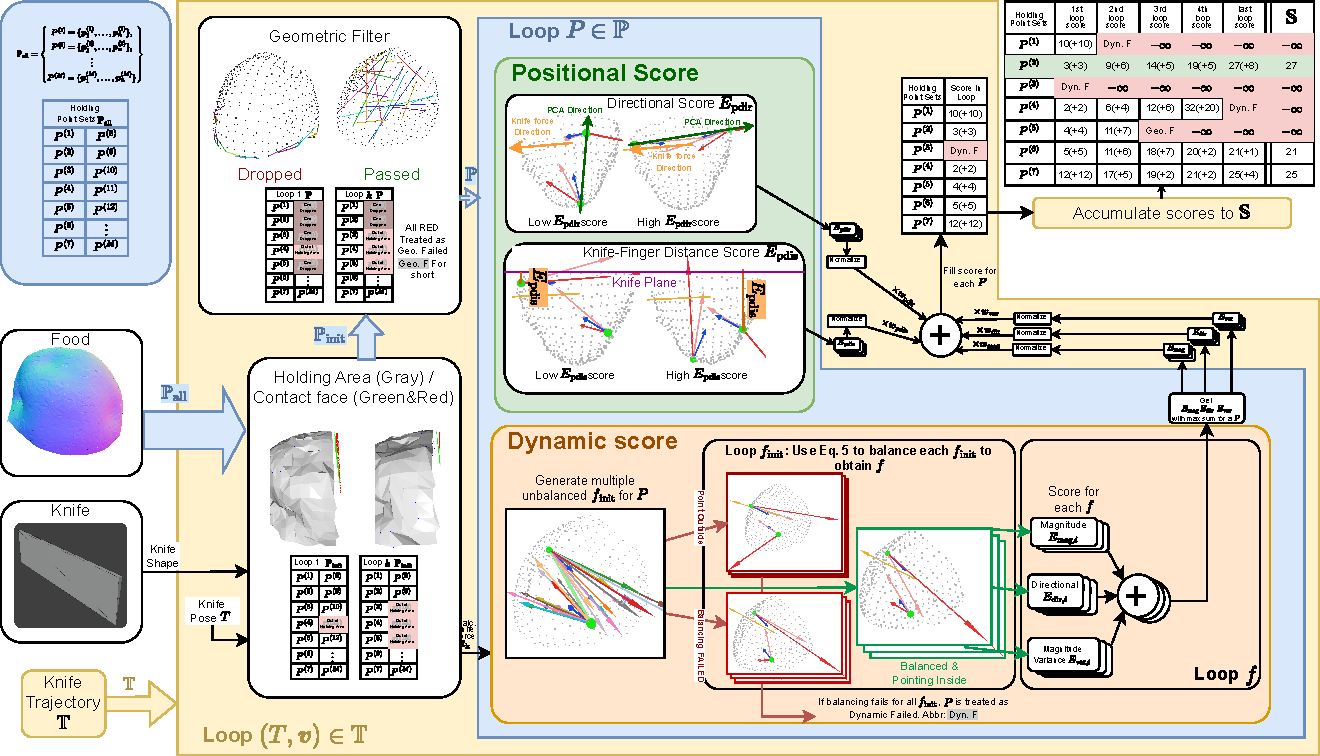
\includegraphics[width=1\linewidth]{fig/chp_holding/SICE2025_AlgoFlow.pdf}
    \caption{ Block diagram of the proposed searching method for the optimal {\nameholdingpointsetENG}. The process takes the food surface, knife mesh, and trajectory $\mathbb{T}$ as inputs. Inside the trajectory loop (yellow area), the search space is initialized and refined via a Geometric Filter. The remaining candidates in $\equsearchspace$ (blue area) are evaluated using Positional Scores (green block) and Dynamic Scores (orange block); the latter selects the best dynamic score of balanced {\namegraspforceENG} $\equgraspforce$ that can resist the knife wrench $\bm{t}_\mathrm{k}$. Finally, the normalized scores are accumulated in $\mathbb{S}$ to identify the final output. }
    \label{fig:holding_Algo1}
\end{figure}



\subsection{幾何フィルタによる{\namesearchspace}の削減}
\label{subsec:holding_geometric_filter}

全{\nameholdingpointset}$\equsearchspace_{\mathrm{all}}$の要素数は点群点数$K$に対して膨大となるため，後続の力学的評価に先立ち，低計算コストな幾何フィルタのみを用いたフィルタリングにより{\namesearchspace}を削減する（アルゴリズム \ref{algo:holding_filter_geo}）．

幾何スコア$S_{\mathrm{geo}}$は，「指同士の距離」「指と包丁の距離」「指の高さ」の3要素の重み付き和として定義される．

「指同士の距離」評価$E_{\mathrm{fin}}$は，二指が過度に接近して実質的に一指として機能することを防ぐために導入される．指間距離が閾値$b$を超えれば最大値1となり，それ以下の場合は指数関数的に減衰する設計とした．具体的には以下の式で定義される．
\begin{align*}
E_{\mathrm{fin}} &= \min_{\substack{i,j=1,\ldots,n\\ i\neq j}}(D(\|\equfingerpoint[][i] - \equfingerpoint[][j]\|))\\
D(x) &=
\begin{cases}
\displaystyle\ \frac{e^{ax/b} - 1}{e^a - 1} & (x \leq b)\\
\ 1 & (\text{otherwise})
\end{cases}
\end{align*}
ここで$a$は減衰の曲率を調整するパラメータ，$b$は指間距離の上限である．

「指と包丁の距離」評価$E_{\mathrm{knf}}$は，包丁の中心平面から各{\namefingerpoint}までの最短距離として定義され，切断動作中の手指と包丁の衝突を防止する役割を担う．
\begin{equation}
E_{\mathrm{knf}} = \min_{i=1,2,\cdots,n}(\mathrm{Dist}(\equfingerpoint[][i], \hat{\bm{n}}_{\mathrm{k}}, \bm{p}_{\mathrm{k}}))
\end{equation}
ここで$\hat{\bm{n}}_{\mathrm{k}}$は包丁平面の法線ベクトル，$\bm{p}_{\mathrm{k}}$は包丁の位置である．

「指の高さ」評価$E_{\mathrm{tbl}}$は，各指先の$z$座標の最小値として定義され，把持点がまな板に近すぎる候補を排除する．
\begin{equation}
E_{\mathrm{tbl}} = \min(p_{1z},\ldots,p_{nz})
\end{equation}

これら3つの評価値を$[0,1]$に正規化した後，重み$w_{\mathrm{fin}}, w_{\mathrm{knf}}, w_{\mathrm{tbl}}$により結合し，上位$\lfloor rN\rfloor$件の候補のみを後段へ出力する．
\begin{equation}
    S_{\mathrm{geo}} = w_{\mathrm{fin}} E_{\mathrm{fin}} + w_{\mathrm{knf}} E_{\mathrm{knf}} + w_{\mathrm{tbl}} E_{\mathrm{tbl}}
    \label{equ:holding_score_geo}
\end{equation}
本実験では出力比率$r=0.6$とした．なお，本フィルタでは指先が食材に接触した状態における拘束のみを考慮し，非接触状態から接触に至る指先の移動経路における衝突については考量しない．

\begin{algorithm}[!t]
\caption{Reduce the search space}
\label{algo:holding_filter_geo}
\begin{algorithmic}[1]
  \setlength{\baselineskip}{11pt}
  \Function{FilterByGeoScore}{$\mathbb{P}$, $T$}
  \State $N$: the number of elements in $\mathbb{P}$
  \State $P_1,\ldots,P_N$: each element of $\mathbb{P}$
  \State $w_\mathrm{fin}, w_\mathrm{knf}, w_\mathrm{tbl}$: weights
  \State \fix[$\mathbb{S}_\mathrm{geo}$: Local map for geometric scores, initialized empty]
  \State $r$: output ratio ($r\in(0, 1]$)
  \For{$i\gets 1, N$}
    \State $E_{\mathrm{fin}, i}\gets E_\mathrm{fin}$ for $P_i$
    \State $E_{\mathrm{knf}, i}\gets E_\mathrm{knf}$ for $P_i$
    \State $E_{\mathrm{tbl}, i}\gets E_\mathrm{tbl}$ for $P_i$
  \EndFor
  \State $\{E_{\mathrm{fin,}i}\}\gets$ \Call{Normalize}{$\{E_{\mathrm{fin,}i}\}$}
  \State $\{E_{\mathrm{knf,}i}\}\gets$ \Call{Normalize}{$\{E_{\mathrm{knf,}i}\}$}
  \State $\{E_{\mathrm{tbl,}i}\}\gets$ \Call{Normalize}{$\{E_{\mathrm{tbl,}i}\}$}
  \For{$i\gets 1, N$}
    \State $S_\mathrm{geo}\gets w_\mathrm{fin} E_{\mathrm{fin,}i} + w_\mathrm{knf} E_{\mathrm{knf,}i} + w_\mathrm{tbl} E_{\mathrm{tbl,}i}$ 
    \State \fix[$\mathbb{S}_\mathrm{geo}[P_i] \gets S_\mathrm{geo}$]
  \EndFor
  \State \fix[Sort $\mathbb{S}_\mathrm{geo}$ by values in descending order]
  \State \fix[$\mathbb{P}_\mathrm{out} \gets$ keys of the top $\lfloor rN\rfloor$ entries in $\mathbb{S}_\mathrm{geo}$]
  \State \fix[\textbf{return} $\mathbb{P}_\mathrm{out}$]
\EndFunction\\
\Function{Normalize}{$\{E_i\}$}  \label{algoline:holding_normalize-func}
\State $N$: the number of elements in $\{E_i\}$
\State $M\gets\max(E_1,\ldots,E_N)$
\State $m\gets\min(E_1,\ldots,E_N)$
\ForAll{$E\in\{E_i\}$}
 \State $E\gets (E - m) / (M - m)$
\EndFor
\State \textbf{return} $\{E_i\}$
\EndFunction  \label{algoline:holding_normalize-func-ed}
\end{algorithmic}
\end{algorithm}


\subsection{位置評価スコア}
\label{subsec:holding_positional_score}

本節は図\ref{fig:holding_Algo1}の中上部緑枠の「位置評価スコア」部分について述べる．

位置評価スコア$S_{\mathrm{pos}}$は，{\nameholdingpointset}の幾何的な配置が包丁から加わる力とトルクへの抵抗に適しているかを評価する指標であり，「方向」と「距離」の二要素から構成される（アルゴリズム \ref{algo:holding_score_pos}）．

「方向」評価$E_{\mathrm{pdir}}$は，{\nameholdingpointset}の主成分方向ベクトル$\mathrm{PCA}(\equholdingpointset)$と包丁平面法線$\hat{\bm{n}}_{\mathrm{k}}$の内積に基づいて定義される．
\begin{equation}
E_{\mathrm{pdir}} = 1 - |\mathrm{PCA}(\equholdingpointset) \cdot \hat{\bm{n}}_{\mathrm{k}}|
\end{equation}
主成分方向が包丁平面に平行であるほど高得点となり，これは多方向からの外力に対して有効に抵抗できる把持配置を優先する意図に基づく．

「距離」評価$E_{\mathrm{pdis}}$は，包丁中心平面から各把持点までの距離の最小値に負号を付して定義される．
\begin{equation}
E_{\mathrm{pdis}} = -\min(\mathrm{Dist}(\equholdingpointset, \hat{\bm{n}}_{\mathrm{k}}, \bm{p}_{\mathrm{k}}))
\end{equation}
包丁平面に近い位置で把持すればより小さな{\namefingerforce}でモーメントを打ち消せるという力学的直観を反映した設計である．

両評価値を$[0,1]$に正規化し，重み$w_{\mathrm{pdir}}, w_{\mathrm{pdis}}$により結合することで$S_{\mathrm{pos}}$を得る．
\begin{equation}
    S_{\mathrm{pos,}i} = w_{\mathrm{pdir}} E_{\mathrm{pdir,}i} + w_{\mathrm{pdis}} E_{\mathrm{pdis,}i}
    \label{equ:holding_score_pos_final}
\end{equation}

\begin{algorithm}[!t]
\caption{Calculate the positional score}
\label{algo:holding_score_pos}
\begin{algorithmic}[1]
\setlength{\baselineskip}{11pt}
\Function{CalPositionalScore}{$\mathbb{P}$, $T$}
    \State $N$: the number of elements in $\mathbb{P}$
    \State $P_1,\ldots,P_N$: each element of $\mathbb{P}$
    \State $w_\mathrm{pdir}, w_\mathrm{pdis}$: weights
    \For{$i\gets 1, N$}
        \State $E_{\mathrm{pdir,}i}\gets E_\mathrm{pdir}$ for $P_i$
        \State $E_{\mathrm{pdis,}i}\gets E_\mathrm{pdis}$ for $P_i$ \label{algoline:holding_CalDynamicScore-pos-score}
    \EndFor
    \State $\{E_{\mathrm{pdir,}i}\}\gets$ \Call{Normalize}{$\{E_{\mathrm{pdir,}i}\}$} \label{algoline:holding_score-pos-final-st}
    \State $\{E_{\mathrm{pdis,}i}\}\gets$ \Call{Normalize}{$\{E_{\mathrm{pdis,}i}\}$}
    \For{$i\gets 1, N$}
        \State $S_{\mathrm{pos},i} \gets w_\mathrm{pdir} E_{\mathrm{pdir},i} + w_\mathrm{pdis} E_{\mathrm{pdis},i}$
    \EndFor  \label{algoline:holding_score-pos-final-ed}

    \State \Return $\{S_{\mathrm{pos},i}\}$
\EndFunction
\end{algorithmic}
\end{algorithm}



\subsection{包丁が食材に与える力とトルクの推定}
\label{subsec:holding_knife_wrench}

包丁が食材に及ぼす力学的負荷$\bm{t}_{\mathrm{k}}\in\mathbb{R}^6$は，Muら\cite{method-cutting-fracture}の手法に基づき，食材の破壊靭性に起因する切断力と，包丁側面と食材接触面間に生じる摩擦力の二成分に分解して推定される．

\begin{figure*}[ht]
    \centering
    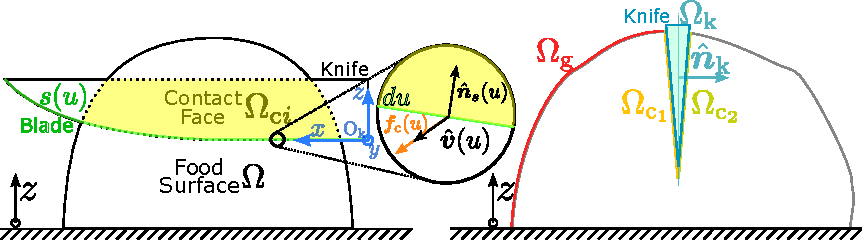
\includegraphics{fig/chp_holding/SICE2025-Method-fig1.pdf}
    \caption{Left: The zoomed-in part shows the calculation of the fracture force due to an infinitesimal element $du$ (in green text and line). Right: The crack generated by the knife creates two contact faces ($\Omega_\mathrm{c_{1}}$ and $\Omega_\mathrm{c_{2}}$). Also, searching only uses one side (the red curve) of the food model.}
    \label{fig:holding_method}
\end{figure*}

\subsubsection{切断力}

包丁の刃曲線を$s(u)$とパラメータ表示し，刃曲線上の位置$u$における包丁面法線ベクトルを$\hat{\bm{n}}_{s}(u)$，速度とその単位方向ベクトルをそれぞれ$\bm{v}(u)$，$\hat{\bm{v}}(u)$とする（図\ref{fig:holding_method}左）．食材の破壊靭性を$\kappa$とすると，位置$u$における微小切断力$\bm{f}_{\mathrm{c}}(u)$は次式で与えられる．
\begin{equation}
\bm{f}_{\mathrm{c}}(u) = -\kappa \left( \hat{\bm{v}}(u) \cdot \hat{\bm{n}}_{s}(u) \right) \hat{\bm{v}}(u)
\end{equation}
これを刃曲線全体にわたって積分することで，食材に作用する全切断力$\bm{f}_{\mathrm{c}}$が求められる．
\begin{equation}
\bm{f}_{\mathrm{c}} = \int \bm{f}_{\mathrm{c}}(u) \, \mathrm{d}u
\end{equation}
また，食材の重心位置$\bm{g}$を用いて，切断力が食材に与えるトルク$\bm{\tau}_{\mathrm{c}}$も併せて計算される．
\begin{equation}
\bm{\tau}_{\mathrm{c}} = \int \left( s(u) - \bm{g} \right) \times \bm{f}_{\mathrm{c}}(u) \, \mathrm{d}u
\end{equation}

\subsubsection{摩擦力}

第\ref{subsec:holding_position}節の仮定に基づき，切断接触面$\Omega_{\mathrm{c}j}$（$j = 1, 2$）に加わる圧力分布は一様（$P_{\mathrm{pres}}$）とする．包丁速度$\bm{v}$を各接触面へ射影した速度成分$\bm{v}_{\mathrm{c}j}$は，接触面の法線ベクトル$\hat{\bm{n}}_{\mathrm{c}j}$を用いて$\bm{v}_{\mathrm{c}j} = \bm{v} - (\bm{v} \cdot \hat{\bm{n}}_{\mathrm{c}j})\,\hat{\bm{n}}_{\mathrm{c}j}$と表される．包丁と食材間の摩擦係数を$\mu$とすると，クーロンの摩擦則に基づく摩擦力$\bm{f}_{\mathrm{fr}}$とトルク$\bm{\tau}_{\mathrm{fr}}$は次式で与えられる．
\begin{align*}
    & \bm{f}_{\mathrm{fr}} = \mu P_{\mathrm{pres}} \sum_{j=1}^2 \iint_{\Omega_{\mathrm{c}j}} \hat{\bm{v}}_{\mathrm{c}j} \, \mathrm{d}S,\\
    & \bm{\tau}_{\mathrm{fr}} = \mu P_{\mathrm{pres}} \sum_{j=1}^2 \iint_{\bm{x} \in \Omega_{\mathrm{c}j}} (\bm{x} - \bm{g}) \times \hat {\bm{v}}_{\mathrm{c}j}\, \mathrm{d}S.
\end{align*}
ここで$S$は接触面$\Omega_{\mathrm{c}j}$の微小面積要素，$\bm{x}$はその中心位置を表す．

\subsubsection{力とトルクの合成}

以上の切断力と摩擦力を6次元ベクトルとして合成した
\begin{equation}
\bm{t}_{\mathrm{k}} = \left[ \left( \bm{f}_{\mathrm{fr}} + \bm{f}_{\mathrm{c}} \right)^{\mathrm{T}}, \left( \bm{\tau}_{\mathrm{fr}} + \bm{\tau}_{\mathrm{c}} \right)^{\mathrm{T}} \right]^{\mathrm{T}}
\label{equ:holding_knife_wrench}
\end{equation}
を，包丁が食材に与える力とトルクとして定義する．


\subsection{{\namegraspforce}候補の効率的生成}
\label{subsec:holding_force_generation}

{\nameholdingpointset}$\equholdingpointset$が定まったとしても，包丁から食材に加わる力とトルク$\bm{t}_{\mathrm{k}}$と釣り合うべき{\namegraspforce}$\equgraspforce\in\mathbb{R}^{3n}$には，把持行列$G$の零空間に起因する無限の冗長性が存在する．

まず，{\namegraspforce}とその合力の関係を定式化する．本研究では指先と食材の接触を点接触と仮定し，指先におけるトルクを無視して各{\namefingerforce}$\equfingerforce[i]$（$i = 1,\ldots, n$）のみを考える．これらを$3n$次元ベクトル$\equgraspforce = [\equfingerforce[1]^{\mathrm{T}},\ldots, \equfingerforce[n]^{\mathrm{T}}]^{\mathrm{T}}$に並べたものを{\namegraspforce}と定義する．{\namegraspforce}$\equgraspforce$が食材に与えた合力を$\bm{t}_{\mathrm{h}} = [\bm{f}_{\mathrm{h}}^{\mathrm{T}}, \bm{\tau}_{\mathrm{h}}^{\mathrm{T}}]^{\mathrm{T}}$とすると，これは包丁の力とトルクと釣り合う必要があり，$\bm{t}_{\mathrm{h}} = -\bm{t}_{\mathrm{k}}$を満たす．

ここで，食材がまな板と安定な平面接触を有し，その運動が$xy$平面内の並進と$z$軸まわりの回転に限定されるという仮定のもとでは，$z$軸方向の力および$x$,$y$軸まわりのトルクはまな板によって相殺される．したがって，必要な合力 $\bm{t}_{\mathrm{h}}$としては力の$x$,$y$成分とトルクの$z$成分のみを考慮すればよく，これを$[f_{\mathrm{h}x}, f_{\mathrm{h}y}, \tau_{\mathrm{h}z}]$と抽出する．

{\namegraspforce}$\equgraspforce$と合力 $\bm{t}_{\mathrm{h}}$の関係は，把持行列$G$を用いて$\bm{t}_{\mathrm{h}} = G \equgraspforce$と表される．把持行列$G$は次の式で定義される$6 \times 3n$行列である．
\begin{equation}
    G = \begin{bmatrix}I_3 & \cdots & I_3 \\ R_1 & \cdots & R_n \end{bmatrix}
    \label{equ:holding_grasp_matrix}
\end{equation}
ここで$I_{3}$は$3 \times 3$の単位行列，$R_{i}$は$\equfingerpoint[][i] - \bm{g}$から構成される歪対称行列であり，$R_i \equfingerforce[i] = (\equfingerpoint[][i] - \bm{g}) \times \equfingerforce[i]$を満たす．実際には，抽出された3成分$[f_{\mathrm{h}x}, f_{\mathrm{h}y}, \tau_{\mathrm{h}z}]$に対応させるため，$G$の3,4,5行目を除いた行列を用いる．この式を$\equgraspforce$について解くと次の式が得られる．
\begin{equation}
    \equgraspforce = G^+ \bm{t}_{\mathrm{h}} + [I_{3n}-G^+ G]\,\bm{k}
    \label{equ:holding_force_balance}
\end{equation}
ここで$G^+$は$G$の擬似逆行列，$\bm{k}$は任意の$3n$次元ベクトルである．$\bm{k}$の選び方により無数の{\namegraspforce}が得られることから，力の冗長性が生じる．

この冗長性に対処するため，本手法ではまず多数の{\namegraspforce}候補を生成し，その中から最適なものを選択する戦略をとる．最も単純な生成法は，式(\ref{equ:holding_force_balance})の任意ベクトル$\bm{k}$に乱数を割り当てる方法である．しかし，このアプローチでは生成された{\namefingerforce}の多くが摩擦円錐の外側を向く，すなわち物理的に妥当でない解となり，生成効率が極めて低い．

そこで提案手法では，二段階の生成方法を提案する．
\begin{enumerate}
    \item 第一段階では，各{\namefingerforce}の方向を摩擦円錐内に限定した初期力$\equgraspforcevector[init]$をランダムに生成する．
    \item 第二段階では，以下の補正式により$\equgraspforcevector[init]$と包丁の力とトルクとの釣り合わない分を補正し，釣り合える{\namegraspforce}$\equgraspforce$を得る．
    \begin{align*}
        \bm{t} &= (-\bm{t}_{\mathrm{k}}) - G \equgraspforcevector[init] \\
        \equgraspforce &= \equgraspforcevector[init] - G^{+}\bm{t}
    \end{align*}
\end{enumerate}

この提案手法により，摩擦円錐内に収まる妥当な{\namegraspforce}候補を，ランダム$\bm{k}$法と比較して平均約7.7倍の効率で生成できることが実験的に確認されている（\ref{subsec:holding_exp_force_generation}節参照）．それでも妥当な{\namefingerforce}が一つも生成できない{\nameholdingpointset}については，無効候補としてスコア$-\infty$を割り当てる．


\subsection{動的評価スコア}
\label{subsec:holding_dynamic_score}

動的評価スコア$S_{\mathrm{dyn}}$は，前節で生成された{\namegraspforce}候補群の中から，力量の大きさ・方向・分散の三基準で最も安定と判定される力を{\nameholdingpointset}ごとに選出し，{\namesearchspace}全体で正規化した評価値である（アルゴリズム \ref{algo:holding_filter_force}）．

動的評価は二段階で構成される．第一段階（ローカル評価）では，単一の{\nameholdingpointset}$\equholdingpointset$に対して生成された全{\namegraspforce}候補を対象に，三基準の重み付きスコアを計算し，最高スコアに対応する力候補のスコアを返す．

力量の大きさ評価$e_{\mathrm{mag}}$は，全{\namefingerforce}のノルム和の負値として定義され，小さな力で把持可能な候補ほど高得点となる．
\begin{equation}
e_{\mathrm{mag}} = - \sum_{i=1}^n \|\equfingerforce[i]\|
\label{equ:holding_emag}
\end{equation}

方向評価$e_{\mathrm{dir}}$は，各{\namefingerforce}ベクトルと接触点における食材表面法線との内積和として定義される．{\namefingerforce}が表面法線方向に近いほど滑りにくいため，この値が大きい候補が優先される．
\begin{equation}
e_{\mathrm{dir}} = \sum_{i=1}^n \hat{\bm{n}}_{\Omega} (\equfingerpoint[][i]) \cdot \hat{\equfingerforce[i]}
\label{equ:holding_edir}
\end{equation}
ここで$\hat{\bm{n}}_{\Omega} (\equfingerpoint[][i])$は食材表面$\Omega$の位置$\equfingerpoint[][i]$における単位法線ベクトルである．

分散評価$e_{\mathrm{var}}$は，各{\namefingerforce}の大きさの分散の負値として定義され，特定の指に力が集中することを避け，全指への均等な負荷分散を促す役割を担う．
\begin{equation}
e_{\mathrm{var}} = - \mathrm{Var}(\|\equfingerforce[1]\|, \|\equfingerforce[2]\|, \dots, \|\equfingerforce[n]\|)
\label{equ:holding_evar}
\end{equation}

これらの三評価値は，一つの{\nameholdingpointset}$\equholdingpointset$に対して生成された全{\namegraspforce}候補間で$[0,1]$にローカル正規化され，重み付き和としてローカルスコア$S$が算出される．
\begin{equation}
    S = w_{\mathrm{mag}} \tilde{e}_{\mathrm{mag,}i} + w_{\mathrm{dir}} \tilde{e}_{\mathrm{dir,}i} + w_{\mathrm{var}} \tilde{e}_{\mathrm{var,}i}
    \label{equ:holding_force_local_score}
\end{equation}
これらのローカルスコア$S$と対応する生素点$\{e_{\mathrm{mag}}, e_{\mathrm{dir}}, e_{\mathrm{var}}\}$がリスト$L$に格納され（アルゴリズム\ref{algo:holding_filter_force}の\ref{algo:holding_force-local-norm-score-st}行），最高の$S$に対応する生素点がローカル段階の出力として返される（アルゴリズム\ref{algo:holding_filter_force}の\ref{algo:holding_force-local-norm-score-ed}行）．

第二段階（グローバル評価）では，ローカル段階で選出された各{\nameholdingpointset}の生素点（$E_{\mathrm{mag}}$, $E_{\mathrm{dir}}$, $E_{\mathrm{var}}$）を{\namesearchspace}$\equsearchspace$全体で$[0,1]$に正規化し，重み付き和として$S_{\mathrm{dyn}}$を算出する．
\begin{equation}
S_{\mathrm{dyn},i} = w_{\mathrm{mag}} \tilde{E}_{\mathrm{mag,}i} + w_{\mathrm{dir}} \tilde{E}_{\mathrm{dir,}i} + w_{\mathrm{var}} \tilde{E}_{\mathrm{var,}i}
\label{equ:holding_force_final_score}
\end{equation}
本実験では，重みを$w_{\mathrm{dir}}=2,\ w_{\mathrm{mag}}=2,\ w_{\mathrm{var}}=1$と設定した．

\begin{algorithm}[!t]
\caption{Algo of the holding score calculation}
\label{algo:holding_filter_force}
\begin{algorithmic}[1]
\setlength{\baselineskip}{11pt}
\Function{CalDynamicScore}{$\bm{t}_\mathrm{k}$, $\equsearchspace$, $\Omega_{\mathrm{g}}$}
    \State $E_{\mathrm{mag,}i} , E_{\mathrm{dir,}i} , E_{\mathrm{var,}i}$: The each part of dynamic score for a $P$

    \For {$i\gets 1, N$}
        \State \fix[$E_{\mathrm{mag,}i} , E_{\mathrm{dir,}i} , E_{\mathrm{var,}i}$ ]
        \State $\quad \gets$ \Call {CalDynamicScoreEach}{$\bm{t}_\mathrm{k}, \equholdingpointset[i] $, $\Omega_{\mathrm{g}}$}
    \EndFor
    
    \State \fix[$\{\tilde{E}_{\mathrm{mag,}i}\}\gets$ \Call{Normalize}{$\{E_{\mathrm{mag,}i}\}$} \label{algo:holding_force-global-norm-score-st} ]
    \State \fix[$\{\tilde{E}_{\mathrm{dir,}i}\}\gets$ \Call{Normalize}{$\{E_{\mathrm{dir,}i}\}$}]
    \State \fix[$\{\tilde{E}_{\mathrm{var,}i}\}\gets$ \Call{Normalize}{$\{E_{\mathrm{var,}i}\}$}] \label{algo:holding_force-global-norm-score-ed}
    
    \For{$i\gets 1, N$}
        \State \fix[$S_{\mathrm{dyn},i} \gets w_\mathrm{mag} \tilde{E}_{\mathrm{mag,}i} + w_\mathrm{dir} \tilde{E}_{\mathrm{dir,}i} + w_\mathrm{var} \tilde{E}_{\mathrm{var,}i}$ ]
    \EndFor
    
    \State \fix[\Return $\{S_{\mathrm{dyn,}i}\}$ \label{algoline:holding_CalDynamicScore-all}]
\EndFunction

\State 

\Function{CalDynamicScoreEach}{$\bm{t}_\mathrm{k}$, $\equholdingpointset$, $\Omega_{\mathrm{g}}$}
    \State \fix[$e_\mathrm{mag},e_\mathrm{dir},e_\mathrm{var}$: Local dynamic score of a generated {\namegraspforceENG}.]
    \State $L$: an empty list
    \State $\fix[Q]$: the number of \fix[\namegraspforceENG] to generate
    \State $[\equgraspforce_\mathrm{1}, \equgraspforce_\mathrm{2}, \dots \equgraspforce_{\fix[Q]}]\gets $\Call {\fix[Generate\namegraspforcetitleENG]}{$\bm{t}_\mathrm{k}, \equholdingpointset$}  
    \label{algoline:holding_CalDynamicScore-GenerateFingerForce-1} \label{algoline:holding_CalDynamicScore-GenerateFingerForce-2} \label{algoline:holding_exp1-ed}
    
    \For{$i\gets 1, \fix[Q]$}
        \State \fix[$e_{\mathrm{mag,}i}\gets $ Calculate $e_{\mathrm{mag}}$ given $\bm{t}_\mathrm{k}, P, \bm{f}_i$ \label{algoline:holding_CalDynamicScore-force-score-st}]
        \State \fix[$e_{\mathrm{dir,}i}\gets $ Calculate $e_{\mathrm{dir}}$ given $\bm{t}_\mathrm{k}, P, \bm{f}_i$ ]
        \State \fix[$e_{\mathrm{var,}i}\gets $ Calculate $e_{\mathrm{var}}$ given $\bm{t}_\mathrm{k}, P, \bm{f}_i$ \label{algoline:holding_CalDynamicScore-force-score-ed}]
    \EndFor \label{algoline:holding_CalDynamicScore-force-score-loop-ed}

    \State \fix[$\{\tilde{e}_{\mathrm{mag,}i}\}\gets$ \Call{Normalize}{$\{e_{\mathrm{mag,}i}\}$} \label{algo:holding_force-local-norm-score-st}]
    \State \fix[$\{\tilde{e}_{\mathrm{dir,}i}\}\gets$ \Call{Normalize}{$\{e_{\mathrm{dir,}i}\}$}]
    \State \fix[$\{\tilde{e}_{\mathrm{var,}i}\}\gets$ \Call{Normalize}{$\{e_{\mathrm{var,}i}\}$} \label{algo:holding_force-local-norm-score-ed}]

    \For{$i\gets 1, M$} \label{algoline:holding_CalDynamicScoreEach-finalscore-st}
        \State \fix[$S_{\mathrm{}}\gets w_\mathrm{mag} \tilde{e}_{\mathrm{mag,}i} + w_\mathrm{dir} \tilde{e}_{\mathrm{dir,}i} + w_\mathrm{var} \tilde{e}_{\mathrm{var,}i}$ ]
        \State \fix[Append $\{S, \{e_{\mathrm{mag,}i},e_{\mathrm{dir,}i},e_{\mathrm{var,}i}\}\}$ to $L$]
    \EndFor

    \State \fix[Find element in $L$ with maximum $S$]
    \State \fix[\Return the raw values $\{e_{\mathrm{mag,}i},e_{\mathrm{dir,}i},e_{\mathrm{var,}i}\}$ of that element.] \label{algoline:holding_sub-return}
    
\EndFunction
\end{algorithmic}
\end{algorithm}


% ------------------------------------------------------------
\section{安定把持ための動作計画・制御}
\label{sec:holding_control}
% ------------------------------------------------------------

% TODO: 重写
\subsection{分析結果から動作指令への変換}
\label{subsec:holding_execution}

前節までの分析により計算された{\nameholdingpointset}$\equholdingpointset[fin]=\{\equfingerpoint[][1],\equfingerpoint[][2]\}$は，食材表面上の目標接触位置を与えるが，それ自体はロボットの動作指令ではない．本節では，この分析結果を双腕ロボットの関節指令へ変換し，把持から切断に至る一連の動作として実行する方法を述べる．

動作制御の流れは，以下の3段階からなる．
\begin{enumerate}
    \item 把持点$\equfingerpoint[][1],\equfingerpoint[][2]$を目標値とし，左腕指ハンドの逆運動学により各指関節角を計算する．
    \item 指先を食材表面へ接触させ，把持を完了する．
    \item 右腕に固定された包丁を，事前計画された切断軌道に沿って動作させる．
\end{enumerate}
このうち，(1)および(2)は分析結果を直接反映する実行段階であり，(3)は分析フェーズにおいて力学的評価の前提条件として参照された包丁軌道そのものを実機上で再現する段階である．


\subsection{把持点への手指配置}
\label{subsec:holding_finger_placement}

実験プラットフォームの詳細は第3章にて述べた通りであり，左腕には食材形状への適応性を重視した3軸2指サーボハンド（図\ref{fig:system:finger-hand}）を，右腕には包丁を固定するための平行グリッパを装着した．

指ハンドの各指はz-y-y-tipの関節構成をとり，FUTABA RS405CBサーボ（最大トルク48.0\,$\mathrm{kgf \cdot cm}$，角度分解能0.1\,deg）により駆動される．{\namefingerpoint}$\equfingerpoint[][i]$から関節角$\bm{q}_i$への変換には，指関節のみのヤコビアン逆運動学を用いた．
\begin{equation}
\Delta\bm{q}_i = J_i^{+}(\bm{q}_i)\, \Delta\equfingerpoint[][i]
\end{equation}
ここで$J_i^{+}$は第$i$指のヤコビアン行列$J_i$の擬似逆行列であり，$\Delta\equfingerpoint[][i]$は現在の{\namefingerpoint}から目標位置$\equfingerpoint[][i]$への変位である．

{\namefingerpoint}制御にはPID制御を用いたが，サーボの駆動電流に設定された不感帯（最大電流の13\%）に起因して，{\namefingerpoint}に最大約1cmの誤差が生じうる点が実装上の制約として残されている．この位置決め誤差は，\ref{subsec:holding_exp_comparison}節で述べる把持安定性評価における外れ値の一因ともなった．


\subsection{包丁軌道の設計と実行}
\label{subsec:holding_knife_trajectory}

切断軌道の設計は，分析フェーズにおける力とトルクの推定（\ref{subsec:holding_knife_wrench}節）と表裏一体の関係にある．包丁の位置姿勢$T$と速度$\bm{v}$の系列$\mathbb{T}$は，把持点探索の入力であると同時に，動作制御フェーズでは右腕が実際に追跡すべき目標軌道となる．

本研究では，Zhouら\cite{Cutting-Slice-1,Cutting-Slice-2}により報告された「包丁を真下に押し込むよりも前後にスライドさせながら切る方が切断に要する力が少なくて済む」という知見に基づき，往復スライス軌道を採用した．軌道は，まな板面に対して25度の角度で下降する二段階構成とした．

%%% TODO: 重新整理这段的意思．
\begin{description}
    \item[前進下降] 包丁を前方かつ下方へ，まな板面から25度の角度で定速下降させる．
    \item[後進下降] 包丁が食材の初期接触高さの半分に達した時点で，方向を反転し，後方かつ下方へ同角度で定速下降させる．
\end{description}

この往復スライス軌道の採用により，単純な押し下げ軌道と比較して切断力が低減される一方で，包丁から食材に加わる力の方向と大きさが時間変化する．提案手法では，アルゴリズム \ref{algo:holding_global}の軌道ループにおいて，各時刻の包丁姿勢$T$と速度$\bm{v}$に対応する力とトルク$\bm{t}_{\mathrm{k}}$を逐次推定し，全時刻を通じて最も安定な{\nameholdingpointset}を探索できる．


\subsection{ロボット動作の実行}
\label{subsec:holding_dual_arm_execution}

把持から切断に至る一連の動作は，以下の手順で実行される．

\begin{enumerate}
    \item 食材（半切りジャガイモまたは玉ねぎ）をまな板上の所定位置に設置する．
    \item RGB-Dカメラにより食材の点群を取得し，3Dモデル$\Omega$を構築する（第3章）．
    \item 提案アルゴリズム（アルゴリズム \ref{algo:holding_global}）により，最適{\nameholdingpointset}$\equholdingpointset[fin]$を探索する．
    \item 切断前の評価用画像を固定カメラにより撮影する．
    \item 左腕指ハンドを$\equholdingpointset[fin]$の各接触点へ誘導し，把持を実行する（\ref{subsec:holding_finger_placement}節）．
    \item 右腕包丁を往復スライス軌道に沿って動作させ，切断を実行する（\ref{subsec:holding_knife_trajectory}節）．
    \item 切断後の評価用画像を固定カメラにより撮影する．
\end{enumerate}

% ------------------------------------------------------------
\section{実験と評価}
\label{sec:holding_experiments}
% ------------------------------------------------------------

\subsection{{\namegraspforce}生成手法の効率性検証}
\label{subsec:holding_exp_force_generation}

\begin{table}[t]
\centering
\caption{The results of generating {\namegraspforceENG}}
\label{tab:holding_exp_generate_force}
\begin{tabular}{cccrcc}
\toprule
\multirow{2}{*}{\shortstack{Point\\Cloud\\No.}} & \multicolumn{2}{c}{Proposed Method} & \multicolumn{2}{c}{Random $\bm{k}$} &  \multirow{2}{*}[-0.5em]{\shortstack{Improve\\\%}}               \\
         \cmidrule{2-3}
         \cmidrule{4-5}
         % \cline{1-5}
         & Passed            & Ratio/\%        & Passed            & Ratio/\%         &  \\
         \midrule
1        & 56661961         & 31.47           & 6918682          & 3.84             & 818.97          \\
2        & 32693962         & 18.16           & 4447361          & 2.47             & 735.13          \\
3        & 71345970         & 39.63           & 9037480          & 5.02             & 789.45          \\
4        & 77728717         & 43.18           & 10174652         & 5.65             & 763.94          \\
5        & 33053551         & 18.36           & 4081123          & 2.27             & 809.91          \\
6        & 77206038         & 42.89           & 10616018         & 5.90             & 727.26          \\
         \midrule
Avg.     & 58115033         & 32.28           & 7545886          & 4.19             & 774.11          \\
\bottomrule
\end{tabular}
\end{table}

提案する{\namegraspforce}生成法の効率性を検証するため，6種類のジャガイモ点群データを用い，提案手法とランダム$\bm{k}$法のそれぞれについて，生成された{\namegraspforce}のうち摩擦円錐内に収まる割合（成功率）を比較した．

実験では，各手法につき試行あたり$1.2\times 10^{5}$個の{\namegraspforce}を生成し，摩擦円錐の頂角は40度，軸方向は接触点における内向き法線ベクトルとした．また，幾何フィルタ後の{\namesearchspace}サイズは上位1500件に固定した．

実験結果を表\ref{tab:holding_exp_generate_force}に示す．提案手法の成功率は平均32.28\%であり，ランダム$\bm{k}$法の平均4.19\%に対して約7.7倍の生成効率を達成した．この結果から，提案手法が物理的に妥当な{\namegraspforce}候補をより効率的に生成できることが確かめられた．


\subsection{把持安定性の比較評価}
\label{subsec:holding_exp_comparison}

\begin{figure}[t]
    \centering
    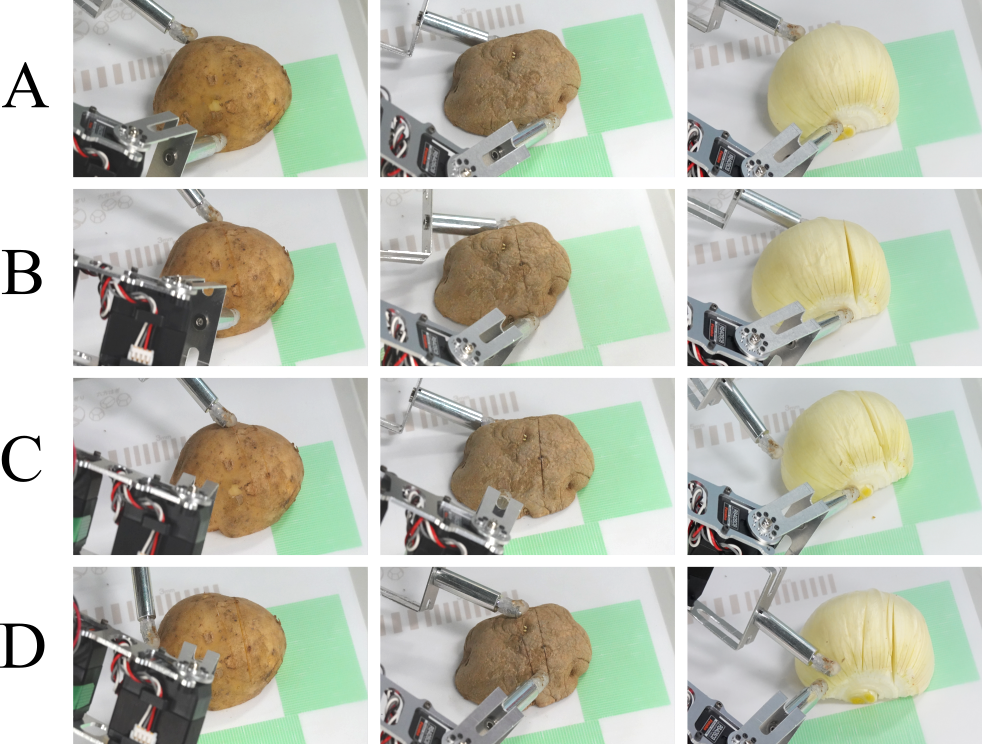
\includegraphics[width=0.85\linewidth]{fig/chp_holding/ICRA2024_HoldingExp.png}
    \caption{Images of the food-stuffs cut by each type of method (in the row).}
    \label{fig:holding_exp_holding_points_type}
\end{figure}

実ロボットによる切断実験では，6個の半切りジャガイモと4個の半切り玉ねぎを対象とし，提案手法（手法A）を含む4種類の把持点選択手法の安定性を比較した．

手法BおよびCは，幾何フィルタ後の上位60\%候補の中から，それぞれ中位および最低位の評価スコアを持つ{\nameholdingpointset}を選択する条件である．手法Dは，幾何フィルタ適用前の全候補$\equsearchspace_{\mathrm{all}}$からランダムに選択する条件である．

各食材は4手法で1回ずつ切断され，切断前後に固定カメラで撮影した画像から食材の平行移動量（pixel）と回転量（deg）を計測することで把持安定性を評価した．なお，同一食材に対する繰り返し切断による切断力の低下を防ぐため，各切断後に計画切断面をその法線方向に2mmずつ移動させた．

実験に用いた食材の物理パラメータは，Muら\cite{method-cutting-fracture}の手法により測定した値を使用した．ジャガイモの破壊靭性は409.66\,J/m$^2$，圧力分布は3352.07\,N/m$^2$，玉ねぎの破壊靭性は646.46\,J/m$^2$，圧力分布は3971.2\,N/m$^2$である．評価関数の重みは，$w_{\mathrm{fin}}=1,\ w_{\mathrm{knf}}=4.4,\ w_{\mathrm{tbl}}=6$，$w_{\mathrm{pdir}}=5,\ w_{\mathrm{pdis}}=4$，$w_{\mathrm{dir}}=2,\ w_{\mathrm{mag}}=2,\ w_{\mathrm{var}}=1$とした．

\begin{table}[H]
\centering
\setlength{\tabcolsep}{3pt}
\caption{Translation (in pixel) \& rotation (in degree) after cutting. The potato cut 6 times, onion cut 4 times.}
\label{tab:holding_exp_result}
\begin{tabular}{ccccccccccc}
\hline
\multirow{2}{*}{\begin{tabular}[c]{@{}c@{}}Holding\\ Type\end{tabular}} &
  \multirow{2}{*}{Food} &
  \multirow{2}{*}{\begin{tabular}[c]{@{}c@{}}Data\\ Type\end{tabular}} &
  \multirow{2}{*}{Avg.} &
  \multirow{2}{*}{Std.} &
  \multicolumn{6}{c}{Oringin Data} \\ \cline{6-11} 
                   &                         &                        &        &                             & 1      & 2      & 3      & 4      & 5      & 6      \\ \hline
\multirow{4}{*}{A} & \multirow{2}{*}{Potato} & \multicolumn{1}{c|}{T} & 113.85 & \multicolumn{1}{c|}{93.13}  & 259.40 & 47.00  & 197.70 & 61.50  & 28.20  & 89.30  \\
                   &                         & \multicolumn{1}{c|}{R} & 3.48   & \multicolumn{1}{c|}{4.30}   & 0.00   & 0.00   & 3.53   & 0.00   & 7.65   & 9.70   \\ \cline{4-11} 
                   & \multirow{2}{*}{Onion}  & \multicolumn{1}{c|}{T} & 84.45  & \multicolumn{1}{c|}{117.06} & 14.40  & 14.80  & 50.40  & 258.20 & ---    & ---    \\
                   &                         & \multicolumn{1}{c|}{R} & 0.99   & \multicolumn{1}{c|}{1.99}   & 0.00   & 0.00   & 0.00   & 3.97   & ---    & ---    \\ \hline
\multirow{4}{*}{B} & \multirow{2}{*}{Potato} & \multicolumn{1}{c|}{T} & 230.03 & \multicolumn{1}{c|}{290.15} & 646.00 & 24.00  & 12.30  & 36.70  & 106.50 & 554.70 \\
                   &                         & \multicolumn{1}{c|}{R} & 5.28   & \multicolumn{1}{c|}{6.36}   & 13.12  & 0.00   & 0.00   & 0.00   & 5.73   & 12.84  \\ \cline{2-11} 
                   & \multirow{2}{*}{Onion}  & \multicolumn{1}{c|}{T} & 41.03  & \multicolumn{1}{c|}{16.49}  & 48.50  & 35.30  & 59.20  & 21.10  & ---    & ---    \\
                   &                         & \multicolumn{1}{c|}{R} & 0.00   & \multicolumn{1}{c|}{0.00}   & 0.00   & 0.00   & 0.00   & 0.00   & ---    & ---    \\ \hline
\multirow{4}{*}{C} & \multirow{2}{*}{Potato} & \multicolumn{1}{c|}{T} & 165.07 & \multicolumn{1}{c|}{191.30} & 526.20 & 76.40  & 114.50 & 21.70  & 222.00 & 29.60  \\
                   &                         & \multicolumn{1}{c|}{R} & 3.85   & \multicolumn{1}{c|}{5.54}   & 14.50  & 0.00   & 2.14   & 5.06   & 1.40   & 0.00   \\ \cline{2-11} 
                   & \multirow{2}{*}{Onion}  & \multicolumn{1}{c|}{T} & 142.90 & \multicolumn{1}{c|}{109.59} & 289.80 & 145.90 & 108.00 & 27.90  & ---    & ---    \\
                   &                         & \multicolumn{1}{c|}{R} & 4.01   & \multicolumn{1}{c|}{5.16}   & 11.45  & 3.43   & 1.15   & 0.00   & ---    & ---    \\ \hline\hline
\multirow{4}{*}{D} & \multirow{2}{*}{Potato} & \multicolumn{1}{c|}{T} & 407.50 & \multicolumn{1}{c|}{198.05} & 759.50 & 304.70 & 263.70 & 520.30 & 345.50 & 251.30 \\
                   &                         & \multicolumn{1}{c|}{R} & 7.69   & \multicolumn{1}{c|}{7.31}   & 16.92  & 1.62   & 3.34   & 8.39   & 15.87  & 0.00   \\ \cline{2-11} 
                   & \multirow{2}{*}{Onion}  & \multicolumn{1}{c|}{T} & 429.70 & \multicolumn{1}{c|}{202.56} & 160.40 & 403.30 & 633.00 & 522.10 & ---    & ---    \\
                   &                         & \multicolumn{1}{c|}{R} & 6.22   & \multicolumn{1}{c|}{3.38}   & 1.28   & 7.25   & 7.39   & 8.96   & ---    & ---    \\ \hline
\end{tabular}
\end{table}

実験結果を表\ref{tab:holding_exp_result}に示す．手法AおよびBは手法CおよびDと比較して明らかに小さな移動量を示し，評価スコアの高い{\nameholdingpointset}ほど安定した把持が実現できることが確認された．

一方で，手法AとBの間には有意な差が見られなかった．これは，幾何フィルタ段階で明らかに不適切な候補が既に排除されており，上位候補はいずれも一定水準以上の安定性を有していたためと考察される．

また，手法AおよびBにおいても一部の試行で大きな移動量（外れ値）が観測されたが，その主因はRGB-Dカメラ点群に残留するノイズによる形状モデルの誤差，およびサーボのPID制御における不感帯に起因する{\namefingerpoint}決め誤差（最大約1cm）であると特定された．

さらに，本実験の評価法そのものにも限界がある．切断前後の画像比較のみでは切断途中の安定性を直接評価できず，往復スライス動作によって切断終了時に食材が元の位置近くに戻された場合，実際には途中で大きく移動していても変位が小さく評価される可能性がある．切断過程全体を通した把持安定性の評価は今後の課題である．


\subsection{完全切断による実用性の実証}
\label{subsec:holding_exp_complete_cut}

\begin{figure}[t]
    \centering
    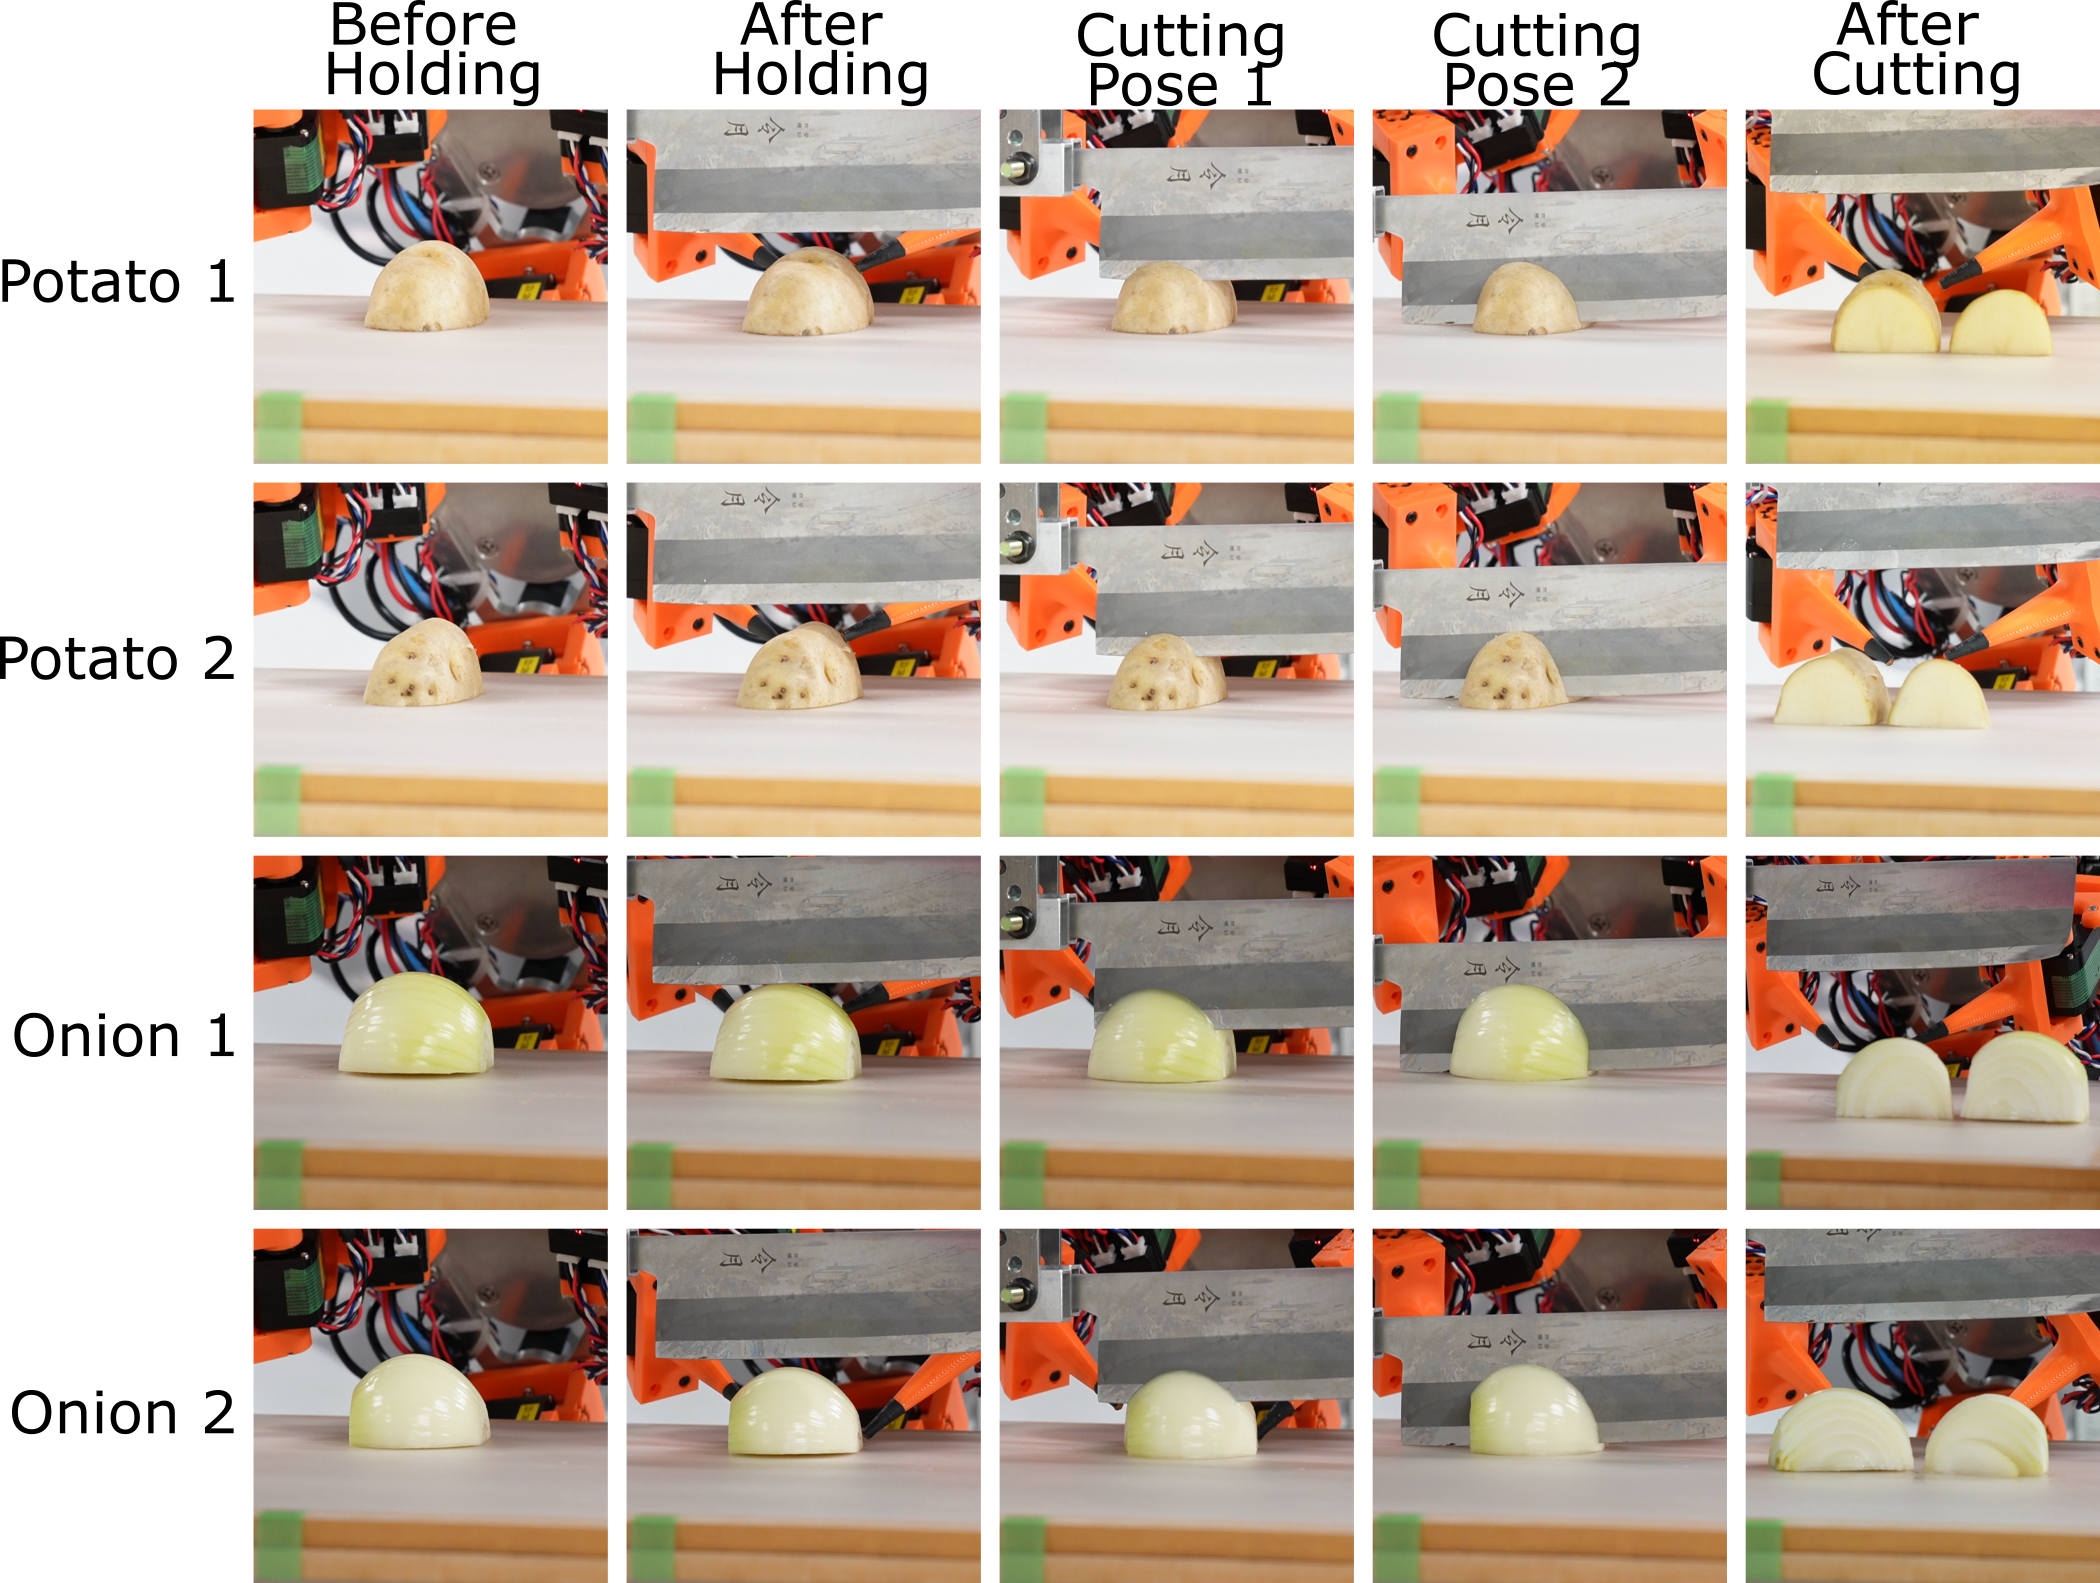
\includegraphics[width=0.95\linewidth]{fig/chp_holding/exp_full_cutting.png}
    \caption{\fix[Snapshots of the cutting process. The rows correspond to different experimental trials with potatoes and onions, while the columns depict the sequential stages of the task (from 'Before Holding' to 'After Cutting').]}
    \label{fig:holding_exp_full_cutting}
\end{figure}

比較実験がサンプル形状保存のための部分切断にとどまるのに対し，本節では食材を完全に切断する実験を行い，提案手法の実用性を検証した．

図\ref{fig:holding_exp_full_cutting}に示す通り，提案手法により選定された{\nameholdingpointset}は，ジャガイモ・玉ねぎのいずれにおいても完全切断の全工程を通じて安定性を維持し，断面の滑らかな切断面が得られた．

\revise{切断中に観測された変位は1\,cm未満であり，把持点での滑りよりもサーボハンドの機械的剛性限界による変形が主因であった．この結果は，平坦面を持つ半切り食材，既知の物性値および包丁軌道という条件下で，食材の大きな移動を防ぎ，滑らかな切断面を伴う完全切断を実行できたことを示す．家庭の食材一般に対する十分性を意味するものではない．}


\subsection{計算コスト分析と実応用に向けた考察}
\label{subsec:holding_exp_computation}

% \begin{table}[H]
%   \centering
%   \caption{\fix[Computation time and score at different point counts.]}
%   % 使用 resizebox 自动缩放表格以适应页面宽度
%   \resizebox{\linewidth}{!}{%
%   \fix[
%   \begin{tabular}{lccccccccc}
%     \toprule
%     \textbf{Point Count} & 7 & 11 & 22 & 62 & 114 & \textbf{169} & 356 & 668 & 1220 \\
%     \midrule
%     \textbf{Time (s)}    & 3.3 & 3.7 & 6.9 & 12.9 & 32.8 & \textbf{75.4} & 283.0 & 995.0 & 3297.7 \\
%     \textbf{Best Score}  & -- & -- & 20.31 & 22.19 & 22.19 & \textbf{22.85} & 22.89 & 22.74 & 22.82 \\
%     \bottomrule
%   \end{tabular}%
% ]
%   % }
% \end{table}
\begin{table}[t]
  \centering
  \caption{\fix[Computation time and score at different point counts.]}
  % 使用 resizebox 自动缩放表格以适应页面宽度
  \label{tab:holding_sensitivity_analysis}
  % \resizebox{\linewidth}{!}
  % {%
  \fix[
  \begin{tabular}{lccccccccc}
    \toprule
    \textbf{Point Count} & 7 & 11 & 22 & 62 & 114 & \textbf{169} & 356 & 668 & 1220 \\
    \midrule
    \textbf{Time (s)}    & 3.3 & 3.7 & 6.9 & 12.9 & 32.8 & \textbf{75.4} & 283.0 & 995.0 & 3297.7 \\
    \textbf{Best Score}  & -- & -- & 20.31 & 22.19 & 22.19 & \textbf{22.85} & 22.89 & 22.74 & 22.82 \\
    \bottomrule
  \end{tabular}%
]
  % }
\end{table}

提案手法の実用展開を見据え，点群密度を7点から1220点まで変化させた際の計算時間と評価スコアの関係を分析した．全計算は，AMD Ryzen 9 3900X 12-Core Processor，64GB RAMを搭載した標準的なPC上で実行した．

実験に採用した約170点の点群密度では平均計算時間は75.4秒であり，評価スコアは約22.85で増加しにくいことが確認された（表\ref{tab:holding_sensitivity_analysis}）．これ以上の点群密度増加はスコア改善にほとんど寄与せず，計算時間のみを増大させる．

\begin{revisionblock}
計算時間の大部分は動的評価スコアの計算（アルゴリズム\ref{algo:holding_filter_force}のCalDynamicScore）が占めており，これは多数の{\namegraspforce}候補を生成・評価する処理に起因する．
現状の実装はオフライン計画を前提とし，約170点でも平均75.4秒を要する．
この待ち時間を家庭内で許容できるかは，並行して行える準備作業や料理工程全体の所要時間に依存するため，本実験だけから十分に許容可能とは結論しない．
力評価処理の並列化，候補点の適応的削減，および再計画頻度の検討が必要である．
\end{revisionblock}

\begin{revisionblock}
\subsection{家庭内の切断作業としての評価}
家庭料理の観点で本章の中心的な成果は，評価スコアそのものではなく，選定した把持点に指を配置することで，半切りのジャガイモと玉ねぎが包丁外力を受けても大きく移動せず，最後まで切断できたことである．
比較実験では，高スコア候補が低スコア・ランダム候補より移動を抑える傾向を示し，完全切断実験では変位を1\,cm未満に保って滑らかな切断面を得た．
この結果により，食材形状を単に認識するだけでなく，既知の切断条件と組み合わせて調理目的に対応する接触位置を決められることを示した．

一方，対象は平坦面を持つ半切り食材二種類であり，丸い食材，柔軟・脆弱な食材，物性が未知の食材には直接適用できない．
包丁軌道と物性値を事前に与える必要があり，計画に約75秒を要し，切断中の変位評価も前後画像を中心としている．
また，指と刃の安全距離は幾何フィルタで扱うが，人共存下の安全，食品衛生，刃物の洗浄は評価していない．
したがって，本章の達成範囲は，設定した食材・接触・物性条件下での安定把持点選択と完全切断である．
\end{revisionblock}


% % ------------------------------------------------------------
% \section{本章のまとめ}
% \label{sec:holding_summary}
% % ------------------------------------------------------------

% 本章では，包丁による食材切断時に生じる外力に対し，食材の意図しない移動を防ぐための{\nameholdingpointset}探索手法を提案した．

% 提案手法の核心は，幾何フィルタによる{\namesearchspace}の効率的削減，包丁が食材に与える力とトルクの力学的推定，{\namegraspforce}の冗長性を考慮した効率的な力候補生成，および大きさ・方向・分散の三基準に基づく動的評価スコアの統合にある．

% 双腕ロボットシステムを用いた実機実験により，提案手法がランダム選択や低スコア候補と比較して有意に高い把持安定性を達成することが示された．さらに完全切断実験により，実用的な切断タスクへの適用可能性も確認された．

% 一方で，現状の手法には平坦な底面を前提とした運動制約，切断前後の画像比較に依存した評価法，および計算時間の制約という限界が残されている．底面が平坦でない食材や球状食材への拡張，切断過程全体を通した把持安定性の評価，および計算の高速化は今後の課題である．



% ------------------------------------------------------------
\section{本章のまとめ}
\label{sec:holding_summary}
% ------------------------------------------------------------

\revise{本章では，食材点群，既知の包丁軌道，指本数，および既知・計測済みの物性値を入力とし，切断中の時間変化するWrenchに抗する{\nameholdingpointset}と指先力を出力するタスク固有の探索手法を構築し，実機で検証した．}
具体的には，以下の分析と制御の流れによって，切断軌道全体にわたる安定把持を実現した．

\begin{enumerate}
	\item \textbf{幾何学的な分析：} RGB-Dカメラで取得した食材の離散点群モデルを用いて{\nameholdingpointset}候補を生成し，指同士の距離・指と包丁の距離・指の高さからなる幾何フィルタによって{\namesearchspace}を効率的に削減した．さらに，{\nameholdingpointset}の主成分方向と包丁平面法線の関係，および各{\namefingerpoint}から包丁平面までの距離を評価する位置評価スコアを設計し，外力に抵抗しやすい幾何配置を優先する仕組みを導入した．
	\item \textbf{力学的な分析：} 食材の破壊靭性と包丁速度に基づき，切断力と摩擦力を統合した時間変化する包丁外力を推定した．また，{\namegraspforce}の冗長性を考慮し，摩擦円錐内に{\namefingerforce}を限定した効率的な力候補生成手法を提案するとともに，{\namefingerforce}の大きさ・方向・分散の三基準による動的評価スコアを局所・大域の二段階で算出し，力学的に最も安定な{\nameholdingpointset}を選出した．
	\item \textbf{動作制御：} 分析により選定された{\nameholdingpointset}$P_{\mathrm{fin}}$に基づき，双腕ロボットの左腕指ハンドを逆運動学により各接触点へ誘導し把持を実行した．その後，右腕に固定した包丁を，分析時に力学的評価の前提として参照した往復スライス軌道に沿って動作させ，分析から制御まで一貫した切断タスクの遂行を可能とした．
\end{enumerate}

実機による検証として，以下の実験を実施し，提案手法の有効性を確認した．
\begin{enumerate}
	\item \textbf{{\namegraspforce}候補の生成効率評価：} 提案する力候補生成手法は，従来のランダム$\bm{k}$法の約4.2\%の成功率に対し，平均32.3\%の成功率を達成し，約7.7倍の効率的な生成を実現した．
	\item \textbf{把持安定性の比較実験：} ジャガイモおよびタマネギを対象に，提案手法（最高スコア）と中位・低スコア・ランダム選択の4条件で比較切断実験を行い，提案手法が高スコア候補は低スコア・ランダム候補に比べて安定する傾向を示したことを確認した．
	\item \textbf{完全切断実験：} 実際に食材を最後まで切断する実験を通じ，提案手法により選定された{\nameholdingpointset}が全工程を通じて安定性を維持し，滑らかな切断面が得られることを実証した．
	\item \textbf{計算コストの分析：} 点群密度と計算時間・評価スコアの関係を調査し，約170点の点群でスコアが飽和し，平均計算時間は約75秒であることを示した．\revise{この時間はオンライン再計画には長く，家庭内での許容性は料理工程全体との関係で別途評価する必要がある．}
\end{enumerate}

一方で，本手法は食材の平坦な底面を前提とした運動制約に依存しており，非平坦な底面への拡張が今後の課題である．
計算の高速化についても，力学的な分析の部分のGPU並列化などによるリアルタイム化が実用化に向けた重要な課題として残されている．
\revise{以上より，幾何情報を候補削減に用い，さらに包丁軌道に沿う力学評価を加えることで，設定条件下では食材移動を抑えて完全切断できる把持点を選定可能になった．ただし，この結論は物性値，包丁軌道，平面接触が与えられる範囲に限定される．}
